% !TEX root = template.tex

% some macros
\newcommand*{\x}{\boldsymbol{x}}
\newcommand*{\y}{\boldsymbol{y}}
\newcommand*{\z}{\boldsymbol{z}}
\newcommand*{\xm}{\bar{\x}}

\section{Processing Pipeline}
\label{sec:processing_architecture}

\begin{figure*}[h]
	\centering
	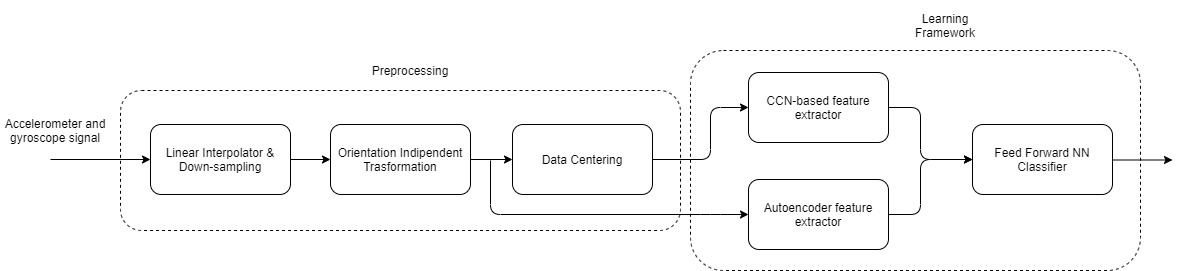
\includegraphics[width=1\textwidth]{images/processing_pipeline.jpg}
	\caption{Processing pipeline}
\end{figure*}

The task of HAR in real use case scenarios is a difficult task, and many aspects need to be considered when these applications are brought in a mobile environment. As reported in \cite{blunck2013heterogeneity} the three major types of heterogeneties which yield impairments in HAR are:
\begin{itemize}
	\item \textbf{Sensor Biases (SB)}: To keep the overall cost of a smartphone low, low costs accelerometer and gyroscope sensor are used, yielding a poor-calibrated, inaccurate an of limited granularity and range acquired signals. So, among this type of sensors we could observe differences in precision, resolution, range and also biases. Usually an initial sensors calibration are made by smartphones manufactures, but due to rotation or misalignment of the sensor to the circuit board of the final product, this could introduce errors. Furthermore, if a device experience shock, e.g falling on the ground, the sensor can be misaligned causing unwanted biases.
	\item \textbf{Sampling Rate Heterogeneity (SRH)}: Often popular smartphones vary in terms of the default and supported sampling frequencies for accelerometer and gyroscope sensor. In the dataset TODO riportare link used for this experiment for example we are dealing with smartphone where the sampling frequency varies from 50Hz to 200Hz. See Fig. TODO so the actual number of devices used in this dataset, with their corresponding sampling frequencies.
	\item \textbf{Sampling Rate Instability (SRI)}: This phenomenon is specific to a single device and regards the regularity of time span between successive measurements. Different factors could accentuate this problem, including heavy multitasking or high I/O load in the mobile device. Multitasking effect in particular is a major problem: smartphone usually prioritizes among various running tasks and doing so could extremely affects the sensor sampling of a HAR application running on the device. In our collected dataset with a 100 Hz sampling rate (which means a time-span between consecutive samples of $10ms$), for example we observe time-span ranging mainly between $3ms$ and $15ms$ with an average of $7ms$. Although in our collected dataset the smartphone was set in \textit{airplane mode} to reduce at minimum this effect. The Fig. \ref{time-span} shows the amount of different time-span present in our dataset.
\end{itemize}

\begin{figure}[h]
	\centering
	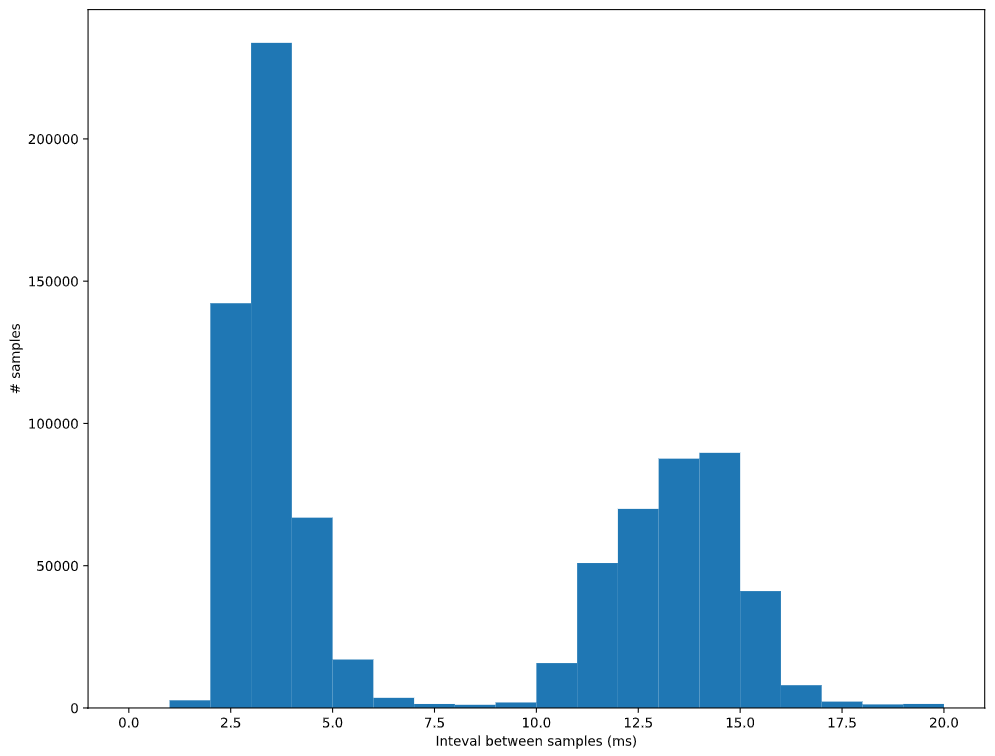
\includegraphics[width=0.4\textwidth]{images/interval_samples.png}
	\caption{Histogram of different time span between samples included in our collected dataset}
	\label{time-span}
\end{figure}

Furthermore, if we considered a real use case scenarios of a HAR mobile application we must also consider that smartphones can be positioned and oriented in different ways in human body. For example a smartphone could lay in trouser pockets (back and front) or maybe inside accessories like in a pouch or in a bag with different orientations. These different initial model settings have huge effects in prediction accuracy of an HAR predictor, especially if the model has been trained on a dataset that consist of activity measurement coming from only one fixed position and orientation of the smartphone, as is usually the case dealing with dataset collected in a controlled environment that could be found on Internet.

To tackle all these problems we decided to adopt in our pre-processing pipeline as show in Fig. TODO, 3 main blocks.

The first block called Linear Interpolator is in charge of mitigate the problems regarding the SRH and SRI as discussed previously. It main purpose is to down-sample the input data to a fixed sampling rate, in our case 50 samples/second.

The second block called Orientation Independent Transformation is used to represent data coming from different orientation of the smartphone in a rotation independent space. In this way all the signals are projected in a new space whose orientation is independent of that of the smartphone and aligned with gravity and the direction of motion. In this way an user can place his smartphone in whatever position he or she wants, mitigating the problem of different position and rotations of smartphone, as we will see in the Experiment section TODO reference.

Our last block consists of a data centering operation, applied for centering signals among y-axis that are presented only for the Covolutional Layer and not for the Autoencoder block. The reason of this choice would be clear in the section TODO. As reported in \cite{ignatov2018real}, time series centering standardize the input data, making the task for the CNN easier. Data normalization instead must be avoided because does not help in this situation since it significantly distorts time series shape, removing magnitude information which is critical for activities differentiation.

After the preprocessing pipeline we adopt a novel Learning framework. It is composed of CNN augmented with features coming from an autoencoder. As discussed in \cite{ignatov2018real} CNNs learns filters that are applied to small sub-regions of the data, and therefore they are able to capture local data pattern and their variations. Additionally, due to a small number of connections and high parallelism the amount of computations and running time of CNNs is significantly lower compared to other deep learning algorithm. This yield these model perfect for real-time HAR apps, where these models could also run in a restrict environment as one like smartphones where computation resources are limited. The only drawback of CCNs is that they fall behind in capturing global properties of the signal, and as proposed in \cite{ignatov2018real} they resolve this problem by augmenting CNNs with some basic statistical features that comprise this aspects of the data. But as opposed to what done in this latter work, where they used manual extracted features, we decided to opt for a autoencoder features extractors which can provide more robust feature. For this reason we train an auto-encoder separately on the training data and then use the encoder part to augment the CNN features used for the last classification Feed Forward Neural Network.

\section{Signals and Features}
\label{sec:model}

Parlare del nostro dataset usato Heterogenity, cioe come sono strutturati i nostri dati partenza.



\subsection{Dataset \& Meausurement Setup}
\label{subsec:dataset-measurement-setup}
Parlare di come abbiamo splittato il dataset, quindi escludendo gli utenti a e b per fare in modo di testare le performance cambiando compltamente utente.

Introduzione e spiegazione del dataset eterogeneo, preso da: riportare link. e riportare come abbiamo tirato fuori le time window con overlapping window!

Accenare dell'acquisizione di un nostro dataset alla stessa maniera, a 100 HZ in varie posizioni per testare poi anche tutto il dataset!

\subsection{Signal preprocessing}

In questo caso si va nel dettaglio (con formule e forse se neccessario anche grafici) della parte di preprocessing (parte trattegiata nel mio schema come preprocessing):

\textbf{Notation}: With $\boldsymbol{x} \in {\rm I\!R}^{n}$ we mean a column vector $\boldsymbol{x}=(x_{1}, x_{2}, ..., x_{n})^{T}$.  With $\boldsymbol{||x||}$ we mean the L2-norm operator $||\x|| = (\sum_{i=1}^{n} x_{i}^{2})^{1/2}$ and with $\bar{x} = (\sum_{i=1}^{n} x_{i}) / n$ the mean of a vector. With $\boldsymbol{x} \cdot \boldsymbol{y} =\boldsymbol{x}^{T}\boldsymbol{y} $ we mean the inner product of two vectors. With $\boldsymbol{\vec{x}}$ we mean a 3D vector $\boldsymbol{\vec{x}} = (x_{1}, x_{2}, x_{3})^{T}$ and with $\boldsymbol{\hat{x}}$ the corresponding 3D versor $\boldsymbol{\hat{x}}=\boldsymbol{\vec{x}}/ ||\boldsymbol{\vec{x}}||$. For any two 3D vector $\boldsymbol{\vec{x}}$ and $\boldsymbol{\vec{y}}$ we indicate their cross-product as $\boldsymbol{\vec{x}} \times \boldsymbol{\vec{y}}$. We represent with $\boldsymbol{a_{x}}, \boldsymbol{a_{y}}, \boldsymbol{a_{z}}$ the x, y and z components of the accellerometer signal, as well as the gyroscope signal is represented with $\boldsymbol{g_{x}}, \boldsymbol{g_{y}}, \boldsymbol{g_{z}}$. We define also matrices with uppercase and bold letters. For example to define a $3 \times n$ matrix composed of 3 vectors \mbox{$\boldsymbol{x}, \boldsymbol{y}, \boldsymbol{z} \in {\rm I\!R}^{n}$} we use the notation \mbox{$\boldsymbol{M} = [\boldsymbol{x}, \boldsymbol{y}, \boldsymbol{z}]^{T}$}\\

\textbf{Linear Interpolation \& Down-sampling}\\

As described in Sec. \ref{subsec:dataset-measurement-setup}, our
dataset is composed by signals collected with different sampling rates
from many mobile phones and they are usually out of sync due to the
SRI. For this reason we apply to all signals a
simple preprocessing pipeline composed by two steps: linear
interpolation and downsampling. With linear interpolation we project
signals with different sampling frequencies, i.e 50, 100, 200 Hz, to a
200 Hz signal TODO: noi non abbiamo piu fatto cosi perche si comporta peggio con i filtri. Linear/nearest interpolation are usually preferred
w.r.t. cubic spline or smooth cubic spline as investigated in
\cite{stisen2015smart}, because they usually mitigate the introduction
of noise or artifacts. In linear interpolation the value at time $t$
is the piecewise-linear interpolation, i.e. the linear interpolation
between the input samples adjacent to $t$ in the sequence of input
sample timestamps. Let $(x_0, y_0)$ and $(x_1, y_1)$ be two known
points, the linear interpolant is the straight line between this
points. For a value $x$ in the interval $(x_0, x_1)$ the value $y$
along the straight line is given from the equation of slopes
\begin{equation}
  \label{eq:linear-interpolation}
  \frac{y - y_0}{x - x_0} = \frac{y_1 - y_0}{x_1 - x_0}.
\end{equation}
It's straightforward now to see that if we need to apply linear
interpolation to a dataset of points we can calculate the \mbox{$x$-s} given
by sampling frequency we want to obtain and then apply the formula
above.

At this point we are ready to downsample. Downsampling allows to
standardize data at fixed sampling frequency in order to extract then
time windows and feature vectors for learning models and, above all,
it reduces noise and artifacts introduced by upsampling. Downsampling
simply disregards points by resampling the signal at a lower frequency
(50 Hz in our case). \footnote{FIXME: Please note that the downsample
  frequency should be a sub-multiple of linear interpolation frequency
  otherwise we could}

\textbf{Orientation Indipendent Transform}\\
To project the signals acquired during an activity in a new space wich is indipendent of the rotation of the smartphone, 3 orthogonal versors need to be found. We decided to adopt the technique proposed in \cite{gadaleta2018idnet}, although many other works proposed a similar solution as in \cite{kunze2009way, henpraserttae2011accurate}. In summary we have to find these 3 orthogonal versor namely vertical versor $\boldsymbol{\hat{v}}$, horizontal versor $\boldsymbol{\hat{h}}$ and lateral versor $\boldsymbol{\hat{l}}$. As the name suggest the vertical versor is aligned with user torso pointing up, the horizontal versor is aligned with the direction of motion, pointing foraward, and the later versor tracks lateral movements and it is othogonal to the other two.

Starting with the vertical versor we need to find where the gravity vector $\boldsymbol{\vec{p}}$ ly in the original space. Although the gravity vector is a constant vector in stationary conditions, during a user activity it continuosly changes in the original cordinate system of the smartphone, therefore we are only able to consider the mean direction of the gravity within the current user activity. So, to estimate it we must considered only the acceleremoter signal: \mbox{$ \boldsymbol{\vec{p}} = (\bar{a_{x}}, \bar{a_{y}}, \bar{a_{z}})^{T}$}  and we now could find the vertical versor with \mbox{$ \boldsymbol{\hat{v}} = \boldsymbol{\vec{p}} / ||\boldsymbol{\vec{p}}|| $}

This is the first axis of our new space, and we can project the datas onto this new versor to obtain the first component axis. To do we define the acceleration matrix \mbox{$\boldsymbol{A} = [ \boldsymbol{a_{x}}, \boldsymbol{a_{y}}, \boldsymbol{a_{z}} ]^{T}$}and the gyroscope matrix \mbox{$\boldsymbol{G} = [ \boldsymbol{g_{x}}, \boldsymbol{g_{y}}, \boldsymbol{g_{z}} ]^{T} $}. Now we could project the data onto $\boldsymbol{\hat{v}}$ by:

\begin{equation}
	\label{v-axis eq}
	 \boldsymbol{a_{v}} = \boldsymbol{A} \cdot \boldsymbol{\hat{v}} ,\;\; \boldsymbol{g_{v}} = \boldsymbol{G} \cdot \boldsymbol{\hat{v}} 
\end{equation}

Now we have to find an horizontal plane, parallel to the floor, where the activity motion mostly occurs. To do so we have to remove the  $\boldsymbol{a_{v}}$ component from the original data. We represent the accelerometer data lying on this new plane as $\boldsymbol{M}$ representing the so called motion plane. To find $\boldsymbol{M}$ we have to: \mbox{$\boldsymbol{M} = \boldsymbol{A} - \boldsymbol{\hat{v}} \boldsymbol{a_{v}}^{T} $}

In this new plane, we could see that the direction with the largest variance of projected data, represents the main direction of motion, ie in which direction the user is currently performing the activity with respect to the current smartphone orientation. By aplying PCA \cite{rao1964use}, we are able to find the direction along which the variance of measurements is maximized. This new extracted vector it is called horizantal vector $\boldsymbol{\vec{h}}$. We now could compute the horizontal versor: \mbox{$ \boldsymbol{\hat{h}} = \boldsymbol{\vec{h}} / ||\boldsymbol{\vec{h}}|| $} and we are now able to project our data onto this second new axis by:

\begin{equation}
	\label{h-axis eq}
	\boldsymbol{a_{h}} = \boldsymbol{A} \cdot \boldsymbol{\hat{h}} , \;\; \boldsymbol{g_{h}} = \boldsymbol{G} \cdot \boldsymbol{\hat{h}}
\end{equation}

To find the last axis its sufficient to apply a cross product between the two last axis found, so $ \boldsymbol{\hat{l}} = \boldsymbol{\hat{v}} \times \boldsymbol{\hat{h}} $ and the obtain our last projection of the original data into this new space by:

\begin{equation}
	\label{l-axis eq}
	\boldsymbol{a_{l}} = \boldsymbol{A} \cdot \boldsymbol{\hat{l}} , \;\; \boldsymbol{g_{l}} = \boldsymbol{G} \cdot \boldsymbol{\hat{l}}
\end{equation}



Combining (\ref{v-axis eq}) (\ref{h-axis eq}) and (\ref{l-axis eq}) lead us to the final accelerometer and gyroscope trasformed vectors lying in this new orientation indipendent space that are $[\boldsymbol{a_{v}}, \boldsymbol{a_{h}}, \boldsymbol{a_{l}}]^T $ and $ [\boldsymbol{g_{v}}, \boldsymbol{g_{h}}, \boldsymbol{g_{l}}]^T $ \\

\textbf{Centering}\\

The last signal processing we perform on the input signal is data
centering. As proved in \cite{ignatov2018real} this could slightly
improve performance within a CNN based learning model because
centering the time series make the task easier for the CNN. We denote with $\x^{c}$ the centered vector of $\x$, ie
\begin{equation}
  \label{eq:centering-func}
  \x^{c} = \x - \bar{x} = (x_1-\bar{x}, x_2-\bar{x},..., x_n-\bar{x})^T.
\end{equation}
Centering is applied for each time-window only on accelerometer data, thus the new centered acceleration matrix:
\begin{equation}
  \label{eq:centering-accelerometer-data}
  \boldsymbol{A}^{c} = [\boldsymbol{a_{x}}^{c}, \boldsymbol{a_{y}}^{c}, \boldsymbol{a_{z}}^{c}]^T
\end{equation}
Please note that we simply apply centering and not normalization which is common in CNN applications because normalization removes relevant information like magnitude which is critical for activities differentiation.

\subsection{Feature vector}
\label{subsec:feature-vector}

TIME WINDOWS

When dealing with time-based signals (or time-series in general) we
must keep in mind that correlation between samples occurs and we have
to handle this useful information. However, in the domain of LAR, even
if samples can be correlated in time, the correlation do not persist
over a long period. In literature many time window intervals were
experimented CITE, CITE and they discovered that the best time window
interval is from $1$s to $2.5$s. For this reason we segment the input
signal in many time windows, each of $2.5$s. A time window of $2.5$s
sampled at $50$Hz leads to $125$ samples per window, which could be
expensive in term of raw data TODO non l'ho capita. To tackle this problem we augment
data with the overlapping window technique setting the overlapping
percentage to $50$\%.

FEATURES

Features are the basic elements that every machine learning algorithm
need in order to learn something. Everything fed into a machine
learning algorithm can be considered a feature, but here we use three different type of features targetting different type of information.

\begin{itemize}
\item \textbf{Raw features}. These enables the model to
  learn directly from data and hopefully from it's shape in order
  to generalize and classify activities. Raw features are represented by
  a $6 \text{x} 125$ matrix where rows are accelerometer and gyroscope
  $x$, $y$ and $z$ dimensions while columns are samples over time.
\item \textbf{Manual features}. Manual features take into account the
  statistical mode of the signal and are used in many applications
  CITE UCI e \cite{ignatov2018real} with great results. We exploit
  manual features like mean, variance, sum of the absolute values and
  the histogram of each input data channel computed on local
  time-windows applied only for accelerometer signal $\boldsymbol{a}$. As defined in \cite{ignatov2018real}, we produce a new basic feature vector $\boldsymbol{f_{b}} = (\bar{a_x}, \bar{a_y}, \bar{a_z}, \sigma_{\boldsymbol{a_{x}}}, \sigma_{\boldsymbol{a_{y}}}, \sigma_{\boldsymbol{a_{z}}}, \tilde{a_x}, \tilde{a_y}, \tilde{a_z}, \psi_{\boldsymbol{a_{x}}\boldsymbol{a_{y}}\boldsymbol{a_{z}}}, $ $ \boldsymbol{h}_{\boldsymbol{a_{x}}}^T, \boldsymbol{h}_{\boldsymbol{a_{y}}}^T, \boldsymbol{h}_{\boldsymbol{a_{z}}}^T)^T$
  where for a generic column vector $\x = (x_1, x_2,..., x_n)^T$ with \mbox{$\x^c = (x_1^c, x_2^c,..., x_n^c)^T$:}
  \begin{align}
    \sigma_{\x} &= \sqrt{  \frac{\sum_{i=1}^{n}(|x^c_i|)^2}{n} } \\
    \tilde{x} &= \frac{\sum_{i=1}^{n}(|x^c_i|)}{n} \\
    \psi_{\x\y\z} &= \frac{\sum_{i=1}^{n} \sqrt{x_i^2 + y_i^2 + z_i^2}} {n}
  \end{align}
  and $\boldsymbol{h}_\x$ is python function that sort the values of $\x$ into 10 equally spaced bins along the x-axis between the minimum and maximum values of $\x$. This lead to a basic features vector composed of 40 manual extracted features.
\item \textbf{Auto-encoder features}. Auto-encoder features are
  automatically extracted from the signal. The auto-encoder as
  described in Sec. TODO is capable to compress data and learn a good
  representation of features keeping only interesting data. The code
  size we use is made up of 36 features features.
\end{itemize}

\section{Learning Framework}
\label{sec:learning_framework}

\begin{figure*}[h]
	\centering
	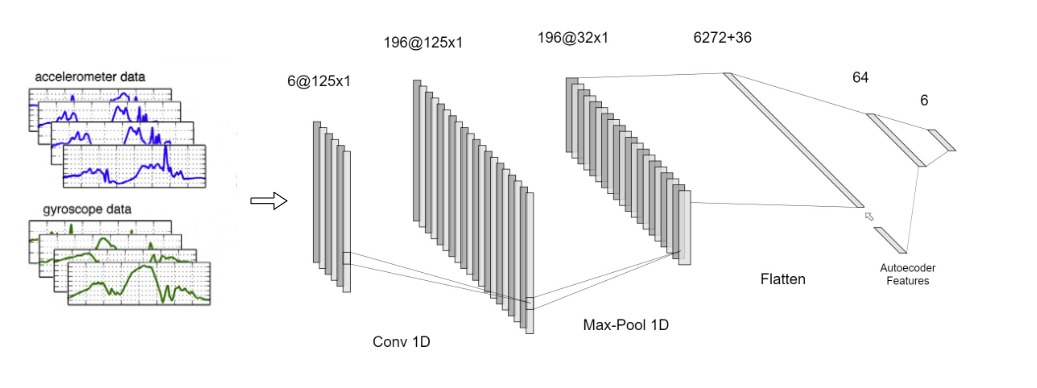
\includegraphics[width=1\textwidth]{images/full_architecture.jpg}
	\caption{Learning Framework}
\end{figure*}

Desctivere qui invece la parte tratteggiata come learning framework

Descivere prima l'autoencoder, come è stato costruito e come viene allenato. TODO luca

Passare alla decrizione della mia archittetura, come sono stai selezionati gli iper-parametri, ecc ecc.
